%This is a test file to determine the layout of the Owl Datasheet
\documentclass{article}
\pagestyle{myheadings}
\markright{BBa\_pSB1K3}
\usepackage[xcolor]{mdframed} %Top header has banner!
\usepackage{hyphenat} %Column titles are not to have hyphenation
\usepackage{seqsplit} %Manages long DNA sequence line breaks
\usepackage{ccaption} %Formatting table titles
\usepackage[margin=1in]{geometry} %Setting document margins
\usepackage{graphicx} %Using images
\usepackage{array} %Formatting table size and behavior
\begin{document}
\renewcommand{\topfraction}{0.99} %Helps with keeping whitespace to a minimum
\renewcommand{\textfraction}{0.99}
\renewcommand{\floatpagefraction}{0.99}
\begin{table}[htbp]
\setlength{\belowcaptionskip}{4pt}
\setlength{\extrarowheight}{8pt}
\begin{mdframed}[backgroundcolor=gray!32,topline=false,rightline=false,leftline=false,bottomline=false] \legend{\Huge \underline{BBa\_pSB1K3}} \end{mdframed} \hfill \break
\begin{tabular}{m{1.2in}m{4.98in}}
\large \textbf{\nohyphens{Part Summary}} & This is a high copy plasmid for use in assembly of BioBrick standard biological parts.\\
\large \textbf{\nohyphens{Part Type}} & Basic Part\\
\large \textbf{\nohyphens{Related Parts}} & pSB1C3, pSB1A3\\
\large \textbf{\nohyphens{Pigeon Image}} & \hfill \break 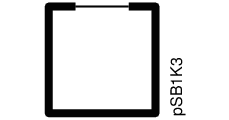
\includegraphics[width=10cm,height=10cm,keepaspectratio]{/Users/Zach/Documents/Owl/igem-datasheet/Datasheet_Generator/src/main/webapp/tmp/1439916876202BBa_pSB1K3_pigeon.png} \\ 
\large \textbf{\nohyphens{Plasmid Map}} & \hfill \break 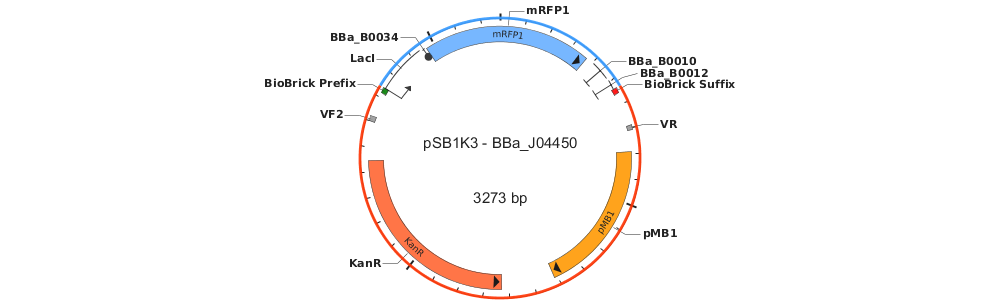
\includegraphics[width=10cm,height=10cm,keepaspectratio]{/Users/Zach/Documents/Owl/igem-datasheet/Datasheet_Generator/src/main/webapp/tmp/1439916876439BBa_pSB1K3_plasmid_map.png} \
\end{tabular}
\end{table}
\begin{table}[htbp]
\setlength{\belowcaptionskip}{4pt}
\setlength{\extrarowheight}{8pt}
\begin{mdframed}[backgroundcolor=gray!32,topline=false,rightline=false,leftline=false,bottomline=false] \legend{\LARGE Designer Information}\end{mdframed}
\begin{tabular}{m{1.2in}m{4.98in}}
\large \textbf{\nohyphens{Author(s)}} & Austin Che\\
\large \textbf{\nohyphens{Date}} & \seqsplit{2008-09-08}\\
\large \textbf{\nohyphens{Contact}} & iGEM HQ
\end{tabular}
\end{table}
\end{document}
